%%%%%%%%%%%%%%%%%%%%%%%%%%%%%%%%%%%%%%%%%%%%%%%%%%%%%%%%%%%%%%%%%%%%%%%
% Project Name : HyperPath                                            %
% Project Home : https://github.com/TeamAC/HyperPath                  %
% Part         : Project architecture                                 %
% Author       : chedi                                                %
% Comments     :                                                      %
%                                                                     %
%%%%%%%%%%%%%%%%%%%%%%%%%%%%%%%%%%%%%%%%%%%%%%%%%%%%%%%%%%%%%%%%%%%%%%%

\section{General Architecture}
Because of the inner nature of the application and the interactions with both
mobile devices and heavy clients, the client-server architecture had been
adopted for this project. The datbase and datawarehouse being used to store the
platform data, we made the choice of having the Java\texttrademark server inbetween
the final consumer and the data. The GlassFish server, can by that wait serve
both the heavy backoffice client\footnote{In our case the heavy backoffice
clinet can became a thin one if we choose to convert the RCP client to RAR} and
the mobile user interface.

In the server, various Beans are affected to the main tasks of:
\begin{description}
  \item[Data administraction] All C.R.U.D operations, import/export of data and
  users and clients managements.
  \item[Services discovery] These are the web services consumed via the mobile
  devices plus the data collected by the tracker mode.
  \item[Recommender] This part is the most important of the application in term
  of complexity and resources usage. The idea here is to have an algorithm
  search the datawarehouse and try to rationalyse the client behaviours, once
  this is done, the services best matching this behvious are collected and a
  recommendation is issued via mail or sms.\footnote{Because this operation
  require a certain amount of dataset and is present a heavy load on the
  system, it's executed in batch mode at night so the client recomendation
  could be send early in the morning, but we're thinking of a better way of
  doing this.}
\end{description}

Some of the WebServices are shared between the Beans, this is totaly normal
because of the fact that the administration Backoffice can be used as the client
to acces the services searchs and recomender feeds\footnote{In general for
testing reason or to select a specific item for update}. To satisfy the
constraints of separation of services, we implement security checks for some web
services and restrict them to validly authentificated
clients.

\begin{figure}[!htb]
  \begin{center}
  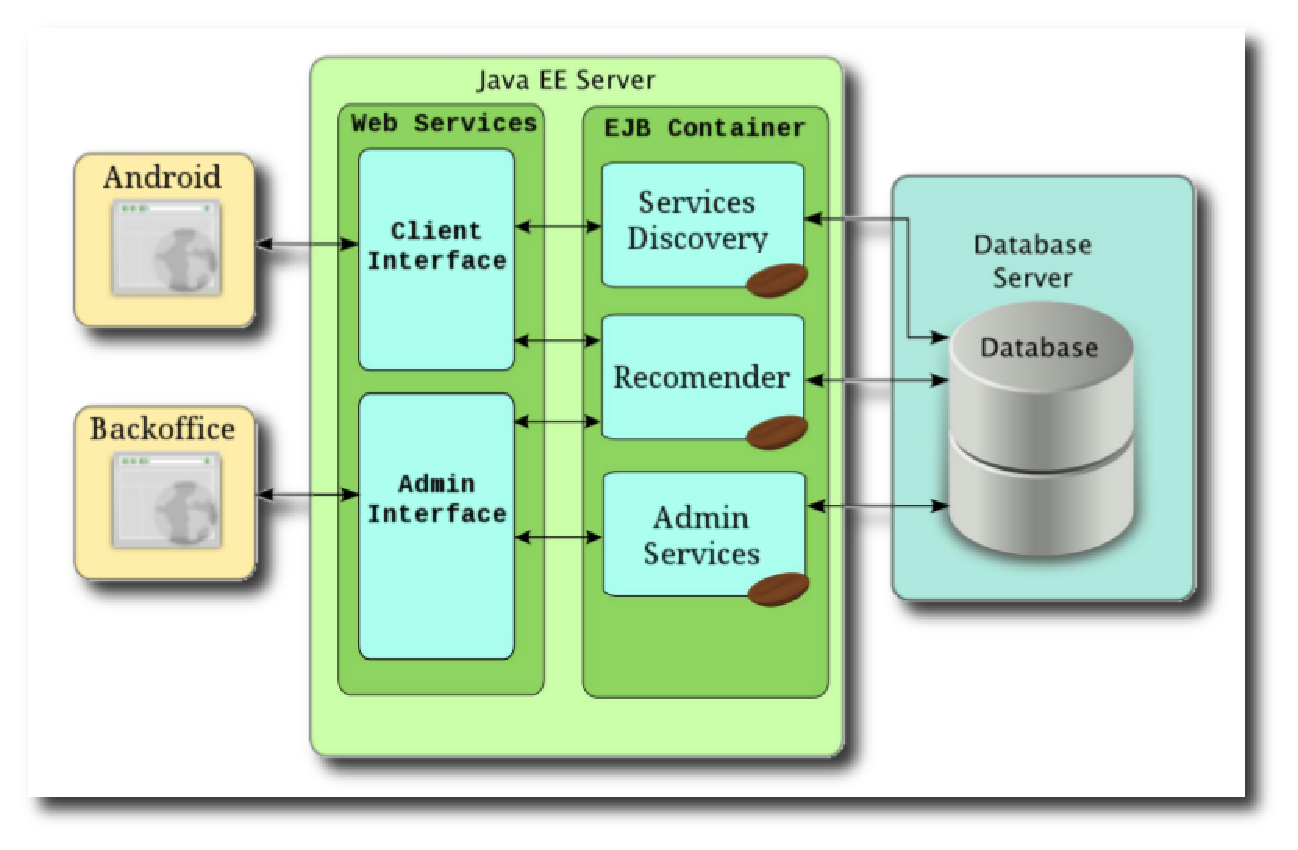
\includegraphics[scale=0.6]{Figures/Architecture_of_HyperPath_Application.eps}
  \end{center}
  \caption{General application architecture}
  \label{General application architecture}
\end{figure}

\section{Application Server}

\section{JEE}
\subsection{Entities}
\subsection{Persistence}
\subsubsection{Object-Persistence}
Java-to-data source integration is a widely underestimated problem when creating
enterprise Java applications. This complex problem involves more than simply
reading from and writing to a data source. The data source elements include
tables, rows, columns, and primary and foreign keys. The Java and Java EE
elements include entity classes, business rules, complex relationships, and
inheritance. In a nonrelational data source, you must match your Java entities
with EIS records or XML elements and schemas. These differences (as shown in the
following figure) are known as the object-persistence impedance mismatch.

\begin{figure}[!htb]
  \begin{center}
  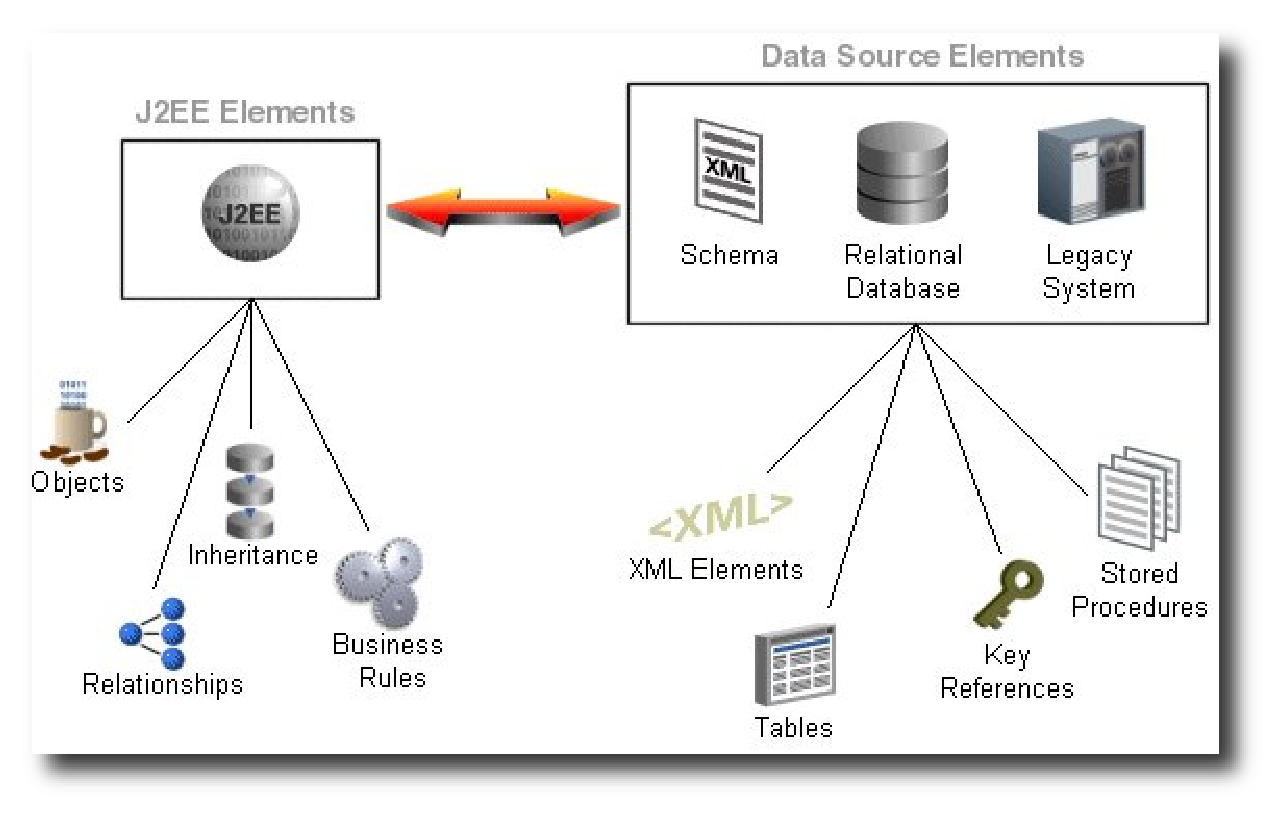
\includegraphics[scale=0.6]{Figures/Object_Persistency_Mismatch.eps}
  \end{center}
  \caption{Solving Object-Persistence Impedance Mismatch}
  \label{Solving Object-Persistence Impedance Mismatch}
\end{figure}

\subsubsection{What Is Java Persistence API?}
\paragraph{}
The Java Persistence API (JPA) is a lightweight framework for Java persistence
based on Plain Old Java Object (POJO). JPA is a part of EJB 3.0 and 3.1
specifications. JPA provides an object relational mapping approach that lets you
declaratively define how to map Java objects to relational database tables in a
standard, portable way. You can use this API to create, remove and query across
lightweight Java objects within both an EJB 3.0/3.1-compliant container and a
standard Java SE 5/6 environment.

JPA includes the following concepts:

\begin{itemize}
\item Entity–any application-defined object with the following characteristics can be an entity:

\begin{itemize}
\item it can be made persistent

\item it has a persistent identity (a key that uniquely identifies an entity
instance and distinguishes it from other instances of the same entity type. An
entity has a persistent identity when there is a representation of it in a data
store)

\item it is partially transactional in a sense that a persistence view of an
entity is transactional (an entity is created, updated and deleted within a
transaction, and a transaction is required for the changes to be committed in the
database). However, in memory entities can be changed without the changes being
persisted.
\item it is not a primitive, a primitive wrapper, or built-in object.
An entity is a fine-graned object that has a set of aggregated state that is
typically stored in a single place (such as a row in a table), and have
relationships to other entities.
\end{itemize}

\item Entity metadata–describes every entity. Metadata could be expressed as
annotations (specifically defined types that may be attached to or place in front
of Java programming elements) or XML (descriptors).
\item Entity manager–enables
API calls to perform operations on an entity. Until an entity manager is used to
create, read, or write an entity, the entity is just a regular nonpersistent Java
object. When an entity manager obtains a reference to an entity, that entity
becomes managed by the entity manager. The set of managed entity instances within
an entity manager at any given time is called its persistence context–only one
Java instance with the same persistent identity may exist in a persistence
context at any time.

You can configure an entity manager toq be able to persist or manage certain
types of objects, read or write to a particular database, and be implemented by a
specific persistence provider. The persistence provider supplies the backing
implementation engine for JPA, including the EntityManager interface
implementation, the Query implementation, and the SQL generation.Entity managers
are provided by an EntityManagerFactory. The configuration for an entity manager
is bound to the EntityManagerFactory, but it is defined separately as a
persistence unit. You name persistence units to allow differentiation between
EntityManagerFactory objects. This way your application obtains control over
which configuration to use for operations on a specific entity. The configuration
that describes the persistence unit is defined in a persistence.xml file.

The following description expresses relationships between JPA concepts:
\begin{itemize}
\item Persistence creates one or more EntityManagerFactory objects
\item each EntityManagerFactory is configured by one persistence unit
\item EntityManagerFactory creates one or more EntityManager objects
\item One or more EntityManager manages one PersistenceContext
\end{itemize}
\end{itemize}
\subsubsection{EclipseLink}
\paragraph{}
EclipseLink is an advanced, object-persistence and object-transformation
framework that provides development tools and run-time capabilities that reduce
development and maintenance efforts, and increase enterprise application
functionality. Using EclipseLink, you can integrate persistence and
object-transformation into your application, while staying focused on your
primary domain problem. EclipseLink addresses the disparity between Java objects
and data sources. EclipseLink is a persistence framework that manages
relational, object-relational data type, EIS, and XML mappings in a seamless
manner. This lets you rapidly build applications that combine the best aspects
of object technology and the specific data source. EclipseLink lets you do the following:

\begin{itemize}
\item Persist Java objects to virtually any relational dqatabase supported by a
JDBC-compliant driver.
\item Persist Java objects to virtually any nonrelational data source supported
by a Java EE Connector architecture (JCA) adapter using indexed, mapped, or XML
enterprise information system (EIS) records.
\item Perform in-memory conversions between Java objects and XML Schema (XSD)
based XML documents using JAXB.
\item Map any object model to any relational or nonrelational schema, using
EclipseLink and JPA integration with several tools including Eclipse Dali,
Oracle JDeveloper, or NetBeans. The Workbench, a graphical mapping tool, is also
provided for backward compatibility for projects using the EclipseLink native API.
\end{itemize}

\section{Web services}
\subsection{Considering Web Services Architecture}
A Web services architecture is similar to the Three-Tier Architecture or Session
Bean Architecture architecture, however, in a Web services architecture, you
encapsulate business logic (the service) in a Web service instead of (or in
addition to) using session beans. In a Web services architecture, clients
communicate with your application using SOAP messages (XML over HTTP).

\begin{figure}
  \begin{center}
  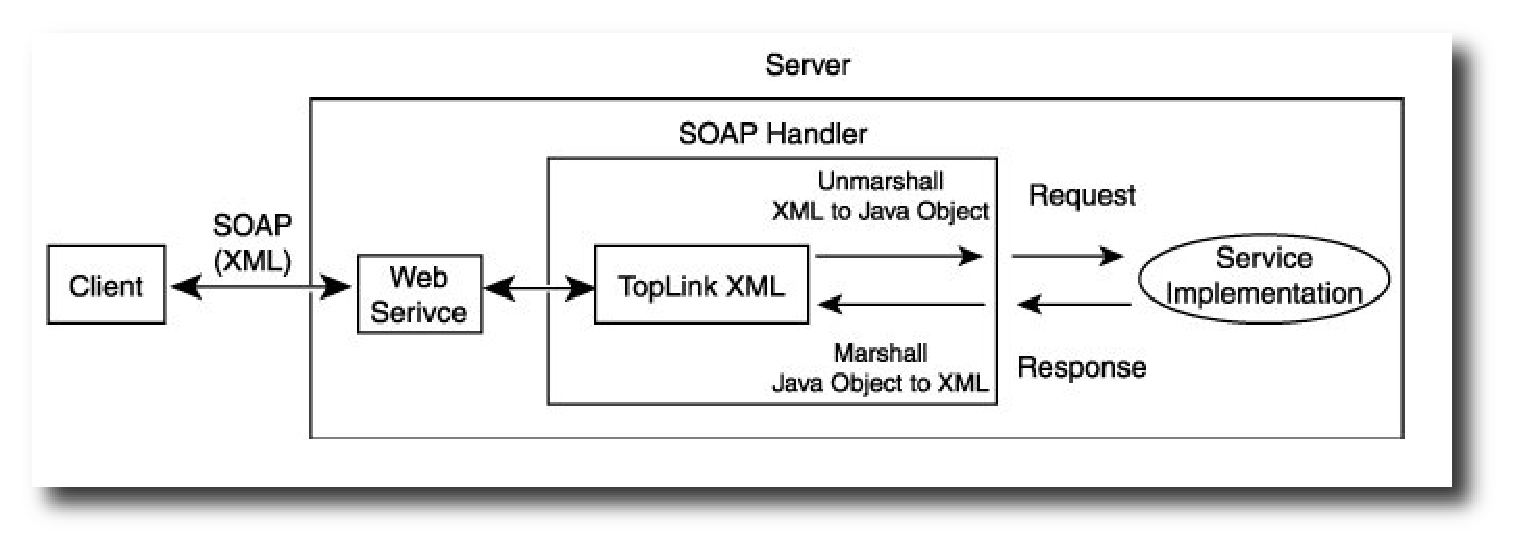
\includegraphics[scale=0.6]{Figures/Web_Service_Arch.eps}
  \end{center}
  \caption{Web Services Architecture}
  \label{Web Services Architecture}
\end{figure}

As in any architecture, you can use EclipseLink to persist objects to relational
or EIS data sources. However, in a Web services architecture, you can also use
EclipseLink to map your object model to an XML schema for use with the Web
service or as the Web service XML serializer.
